%!TEX root = ../main.tex
%
\section{Ball and plate}
%
\begin{frame}
\frametitle{Ball and plate}
%
\begin{figure}
		{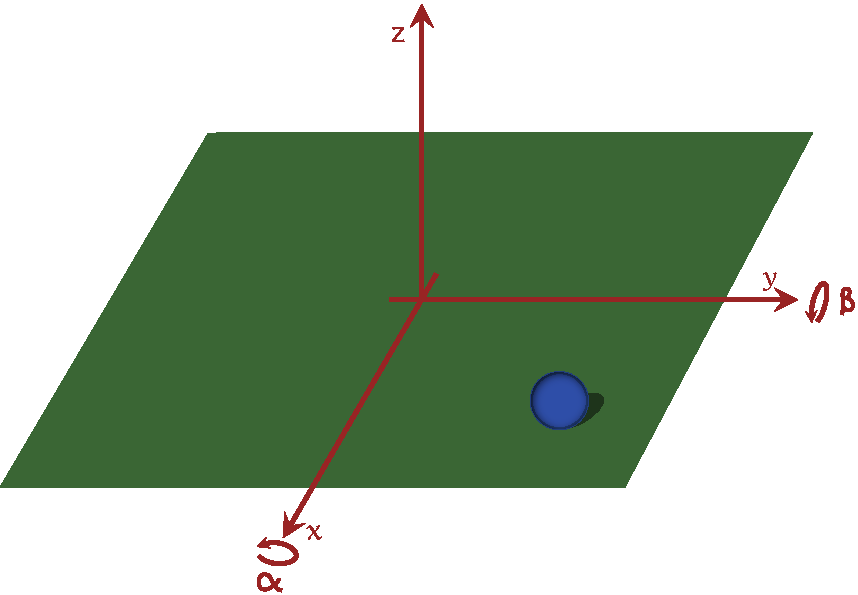
\includegraphics[width=.8\linewidth]{img/ballplate.pdf}}
		\caption{Coordinate frame of the ball and plate system}
		\label{fig:BallPlate}
\end{figure}
\end{frame}
%
\begin{frame}
\frametitle{Ball and plate - Parameters}
\begin{table}
\begin{center}
\begin{tabu} to \textwidth { | X[c] | X[c] | X[c] | }
	\hline
	\textbf{Parameter} & \textbf{Description} & \textbf{Value} \\
	\hline
	$m$ & Mass of the ball & $0.0109 \, Kg$ \\
	$r$ & Radius of the ball & $0.01 \, m$ \\
	$I_b$ & Ball inertia & $4.3563e^{-7} \, Kg\times m^2$ \\
	$l_p$ & Plate side & $0.6 \, m$ \\
	$I_p$ & Plate inertia & $0.175 \, Kg\times m^2$ \\
	\hline
\end{tabu}
\caption{Ball and plate geometric and dynamic parameters}
\label{tab:BallPlate_param}
\end{center}
\end{table}
\end{frame}
%
\subsection{Dynamic}
\begin{frame}
\frametitle{Ball and plate - Dynamic model}
%
The general form of Euler-Lagrange for dynamic equations is used to describe the system:
%
\begin{equation}
	\frac{d}{dt}\frac{\delta T}{\delta q_i} - \frac{\delta T}{\delta q_i} + \frac{\delta V}{\delta q_i} = Q_i
\end{equation}
%
Where $T$ is the kinetic energy, $V$ is the potential energy, $Q_i$ is the i-th generalized force and $q_i$ id the i-th generalized coordinate. As generalized force we consider two torques acting on the plate $(Q_\alpha = \tau_\alpha, Q_\beta = \tau_\beta)$. As generalized coordinates we select two ball position coordinates $[x, y]$ on the frame fixed to the plate and two plate inclination $[\alpha, \beta]$.
\end{frame}
%
\begin{frame}
\frametitle{Ball and plate - Dynamic model}
%
Kinetic energy of the ball:
\begin{equation}
	T_{b} = \frac{1}{2}mv^2 + \frac{1}{2}I_b\omega^2 = \frac{1}{2}\left(m+\frac{I_b}{r^2}\right)\left(\dot{x}^2+\dot{y}^2\right)
\end{equation}
%
Kinetic energy of the plate:
\begin{equation}
	T_{p} = \frac{1}{2}\left(I_b + I_p\right)\left(\dot{\alpha} + \dot{\beta}\right) + \frac{1}{2}m\left(\dot{\alpha}x + \dot{\beta}y\right)^2
\end{equation}
%
Potential energy:
\begin{equation}
	V = mgh = mg(x\,sin\alpha + y\,sin\beta)
\end{equation}
\end{frame}
%
\begin{frame}
\frametitle{Ball and plate - Dynamic model}
%
After some derivations we find the following non-linear system of equations:
%
\begin{align}
	\left(m + \frac{I_b}{r^2}\right)\ddot{x} &- m\left(\dot{\alpha}\dot{\beta}y + \dot{\alpha}^2x\right)+mg\,sin\alpha = 0 \nonumber \\
	\left(m + \frac{I_b}{r^2}\right)\ddot{y} &- m\left(\dot{\alpha}\dot{\beta}x + \dot{\beta}^2y\right)+mg\,sin\beta = 0 \\
	\left(I_p + I_b + mx^2\right)\ddot{\alpha} &+ m\left(\ddot{\beta}xy + \dot{\beta}\left(\dot{x}y + x\dot{y}\right) + 2\dot{\alpha}\dot{x}x\right) +mgx\,cos{\alpha} = \tau_\alpha \nonumber \\
	\left(I_p + I_b + my^2\right)\ddot{\beta} &+ m\left(\ddot{\alpha}xy + \dot{\alpha}\left(\dot{x}y + x\dot{y}\right) + 2\dot{\beta}\dot{y}y\right) +mgy\,cos{\beta} = \tau_\beta \nonumber
\end{align}
\end{frame}
%
\begin{frame}
\frametitle{Ball and plate - Dynamic model}
%
We express the dynamic in matrix form:
%
\begin{equation*}
\begin{aligned}
M(q) &=%
\begin{pmatrix}
	\left(m + \frac{I_b}{r^2}\right) &0 &0 &0\\
	0 &\left(m + \frac{I_b}{r^2}\right) &0 &0\\
	0 &0 &\left(I_b + I_p + mx^2\right) &mxy\\
	0 &0 &mxy &\left(I_b + I_p + my^2\right)
\end{pmatrix}\\
C(q,\dot{q}) &=%
\begin{pmatrix}
	0 &0 &-\dot{\alpha} x &-\dot{\alpha} y\\
	0 &0 &-\dot{\beta} x &-\dot{\beta} y\\
	2\dot{\alpha}x &0 &0 &\left(\dot{x}y+x\dot{y}\right)\\
	0 &2\dot{\beta}y &\left(\dot{x}y+x\dot{y}\right) &0
\end{pmatrix}\\
G(q) &=%
\begin{pmatrix}
	mg\,sin\alpha\\
	mg\,sin\beta\\
	mgx\,cos\alpha\\
	mgx\,cos\beta
\end{pmatrix}
\end{aligned}
\end{equation*}
\end{frame}
%
\begin{frame}
\frametitle{Ball and plate - Dynamic model}
%
\textbf{Affine-in-control formulation}:
\begin{equation}
	\dot{x} =%
	\begin{pmatrix}
	x_5\\ x_6\\ x_7\\ x_8\\ -B(q)^{-1}\left(C(q,\dot{q})\dot{q}+G(q)\right)
	\end{pmatrix}
	+
	\begin{pmatrix}
		0_{4\times2}\\
		B(q)^{-1}
	\end{pmatrix}
	\begin{pmatrix}
		\tau_1\\
	 	\tau_2
	\end{pmatrix}
\end{equation}
Where
\[x = (x_b, y_b, \alpha, \beta, \dot{x_b}, \dot{y_b}, \dot{\alpha}, \dot{\beta})^T\]
\end{frame}
%
\begin{frame}
\frametitle{Ball and plate - Change of coordinates}
In order to simplify the analysis of the structural properties of the Ball and plate system, the following change of coordinates is adopted:
\begin{align}
	u_1 = 2mx\dot{x}\dot{\alpha} - mgx\,cos\alpha - \left(I_p + I_b + mx^2\right)\ddot{\alpha} - m\dot{\beta}\left(\dot{x}y + \dot{y}x\right) - 2m\dot{\alpha}\dot{x}x \nonumber \\
	u_2 = 2my\dot{y}\dot{\beta} - mgy\,cos\beta - \left(I_p + I_b + my^2\right)\ddot{\beta} - m\dot{\alpha}\left(\dot{x}y + \dot{y}x\right) - 2m\dot{\beta}\dot{y}y \nonumber
\end{align}
\end{frame}
%
\begin{frame}
\frametitle{Ball and plate - Change of coordinates}
We obtain the following system in affine form:
\begin{equation}\label{BP_equations}
\dot{x} =%
	\begin{pmatrix}
	x_5\\
	x_6\\
	x_7\\
	x_8\\
	\mathcal{E}(x_7x_8x_2 + x^2_3x_1 - g\,sinx_3)\\
	\mathcal{E}(x_7x_8x_1 + x^2_3x_2 - g\,sinx_4)\\
	0\\
	0\\
	\end{pmatrix}
	+
	\begin{pmatrix}
		0 &0\\
		0 &0\\
		0 &0\\
		0 &0\\
		0 &0\\
		0 &0\\
		1 &0\\
		0 &1\\
	\end{pmatrix}
	\begin{pmatrix}
		u_1\\
	 	u_2
	\end{pmatrix}
\end{equation}\\[10pt]
Where \[\mathcal{E} = \frac{mr^2_b}{mr^2_b + I_b}\]
\end{frame}
%
\subsection{Structural properties}
\subsubsection{Observability}
\begin{frame}
\frametitle{Observability}
Given the observation space $\mathcal{O}$ as the space containing all the repeated Lie-derivatives:
\[
\mathcal{O} = \left\{h(\bar{x}),\;L_fh(\bar{x}),...\,,L_{g_i}L_fh(\bar{x}),...\right\}
\]
The system results locally observable if $dim\,(d\mathcal{O}) = n$, where $d\mathcal{O}$ is the observability codistribution:
\[
d\mathcal{O} = \left\{\frac{\partial h(\bar{x})}{\partial x},\;\frac{\partial L_fh(\bar{x})}{\partial x},...\,,\frac{\partial L_{g_i}L_fh(\bar{x})}{\partial x},...\right\}
\]
\end{frame}
%
% \begin{frame}
% \frametitle{Observability}% modello semplificato
% \begin{equation*}
% 	d\mathcal{O} =%
% 	\begin{pmatrix}
% 		1 &0 &0 &0 &0 &0 &0 &0 \\
% 		0 &1 &0 &0 &0 &0 &0 &0 \\
% 		0 &0 &0 &0 &1 &0 &0 &0 \\
% 		0 &0 &0 &0 &0 &1 &0 &0 \\
% 	    d\mathcal{O}_{51} &0 &d\mathcal{O}_{53} &0 &0 &0 &d\mathcal{O}_{57} &0 \\
% 		0 &d\mathcal{O}_{62} &0 &d\mathcal{O}_{64} &0 &0 &0 &d\mathcal{O}_{68} \\
% 		0 &0 &d\mathcal{O}_{73} &0 &d\mathcal{O}_{75} &0 &d\mathcal{O}_{77} &0 \\
% 		0 &0 &0 &d\mathcal{O}_{84} &0 &d\mathcal{O}_{86} &0 &d\mathcal{O}_{88} \\
% 		\vdots &\vdots &\vdots &\vdots &\vdots &\vdots &\vdots &\vdots
% 	\end{pmatrix}_{48\times8}
% \end{equation*}
% \end{frame}
%
\begin{frame}
\frametitle{Observability}
\begin{equation*}
	d\mathcal{O} =%
	\begin{pmatrix}
		1 &0 &0 &0 &0 &0 &0 &0 \\
		0 &1 &0 &0 &0 &0 &0 &0 \\
		0 &0 &0 &0 &1 &0 &0 &0 \\
		0 &0 &0 &0 &0 &1 &0 &0 \\
	    \star &\star &\star &0 &0 &0 &\star &\star \\
		0 &0 &\star &0 &0 &0 &\star &\star \\
		0 &0 &\star &0 &\star &\star &\star &\star \\
		0 &0 &0 &\star &\star &\star &\star &\star \\
		\vdots &\vdots &\vdots &\vdots &\vdots &\vdots &\vdots &\vdots
	\end{pmatrix}_{48\times8}
\end{equation*}\\[8pt]
Where $\star$ elements represent non constant terms of $d\mathcal{O}(x)$ matrix.
\end{frame}
%
\begin{frame}
\frametitle{Observability}
In order to calculate $rank(d\mathcal{O})$ we perform the following columns and rows swapping:
\begin{equation*}
columns\;5,6 \leftarrow\rightarrow columns\;3,4
\end{equation*}
We obtain the following matrix:
\begin{equation*}
	d\tilde{\mathcal{O}} =%
	\begin{pmatrix}
		1 &0 &0 &0 &0 &0 &0 &0 \\
		0 &1 &0 &0 &0 &0 &0 &0 \\
		0 &0 &1 &0 &0 &0 &0 &0 \\
		0 &0 &0 &1 &0 &0 &0 &0 \\
	    \star &\star &0 &0 &\star &0 &\star &\star \\
		\star &\star &0 &0 &0 &\star &\star &\star \\
		0 &0 &\star &\star &\star &0 &\star &\star \\
		0 &0 &\star &\star &0 &\star &\star &\star \\
		\vdots &\vdots &\vdots &\vdots &\vdots &\vdots &\vdots &\vdots
	\end{pmatrix}_{48\times8}
\end{equation*}
\end{frame}
%
\begin{frame}
\frametitle{Observability}
Studying the matrix obtained one can see that the first 4 rows are:
\[
\begin{pmatrix}
I &\emptyset
\end{pmatrix}_{4\times8}
\]
It is thus sufficient to append 4 rows to this matrix to find a matrix completion of dimension $n=8$.\\
We find a block matrix in the form:
\begin{equation*}
	d\tilde{\mathcal{O}} =%
	\begin{pmatrix}
		A &B \\
        C &D
	\end{pmatrix}
\end{equation*}\\[8pt]
Given the determinant formula for block matrices: $det(M) = det(A-BD^{-1}C)det(D)$\\[8pt] We can see that it is sufficient to study the submatrix $D$ to conclude on eventual rank deficiency of $d\tilde{\mathcal{O}}$.
\end{frame}
%
\begin{frame}
\frametitle{Observability}
We select the following rows sets $r_i$ of $d\tilde{\mathcal{O}}$:
\begin{itemize}
	\item $r_1 = \{21,22,23,6\} \implies det(D_1)\,=\,-2\,\mathcal{E}^4\,g^2\,{x_{1}}^2\,\cos x_{4}\,\sin x_{3} \implies rank(d\tilde{\mathcal{O}})<8\; \mathit{iff} \;x_1\equiv0\; \lor\; x_3\equiv0\; \lor\; x_4\equiv\pi/2$
	\item $r_2 = \{37,38,5,40\} \implies det(D_2)\,=\,-2\,\mathcal{E}^4\,g^2\,{x_{2}}^2\,\cos x_{3}\,\sin x_{4} \implies rank(d\tilde{\mathcal{O}})<8\; \mathit{iff} \;x_2\equiv0\; \lor\; x_3\equiv\pi/2\; \lor\; x_4\equiv0$
	\end{itemize}
	%
	Case $x_1 \equiv 0 \land x_2 \equiv 0$:
	\begin{itemize}
	\item $r_3 = \{5,6,23,24\} \implies det(D_3)\,=\,2\,\mathcal{E}^4\,g^2\,{x_{5}}^2\,\cos x_{3}\,\cos x_{4} \implies rank(d\tilde{\mathcal{O}})<8\; \mathit{iff} \;x_5\equiv0\; \lor\; x_3\equiv\pi/2\; \lor\; x_4\equiv\pi/2$
	\item $r_4 = \{5,6,39,40\} \implies det(D_4)\,=\,2\,\mathcal{E}^4\,g^2\,{x_{6}}^2\,\cos x_{3}\,\cos x_{4} \implies rank(d\tilde{\mathcal{O}})<8\; \mathit{iff} \;x_6\equiv0\; \lor\; x_3\equiv\pi/2\; \lor\; x_4\equiv\pi/2$
	\end{itemize}
\end{frame}
%
\begin{frame}
\frametitle{Observability}
	Case $x_3 \equiv 0\; \land\; x_4 \equiv 0$:
	\begin{itemize}
	\item $r_5 = \{5,6,23,24\} \implies det(D_5)\,=2\,\mathcal{E}^4\,g^2\,{x_{5}}^2 \implies rank(d\tilde{\mathcal{O}})<8\; \mathit{iff} x_5\equiv0$
	\item $r_6 = \{5,6,39,40\} \implies det(D_6)\,=2\,\mathcal{E}^4\,g^2\,{x_{6}}^2 \implies rank(d\tilde{\mathcal{O}})<8\; \mathit{iff} x_6\equiv0$
	\end{itemize}
	%
	Case $x_1 \equiv 0\; \land\; x_2 \equiv 0\; \land\; x_5 \equiv 0\; \land\; x_6 \equiv 0\;$:
	\begin{itemize}
	\item $r_7 = \{5,6,7,8\} \implies det(D_7)\,=\mathcal{E}^4\,g^4\,{\cos x_{3}}^2\,{\cos x_{4}}^2 \implies rank(d\tilde{\mathcal{O}})<8\; \mathit{iff} x_3\equiv\pi/2\; \lor\; x_4\equiv\pi/2$
	\end{itemize}
	%
	Case $x_3 \equiv 0\; \land\; x_4 \equiv 0\; \land\; x_5 \equiv 0\; \land\; x_6 \equiv 0\;$:
	\begin{itemize}
	\item $r_8 = \{5,6,7,8\} \implies det(D_8)\,=\mathcal{E}^4\,g^4 \implies rank(d\tilde{\mathcal{O}})<8\; \mathit{iff} x_3\equiv\pi/2\; \lor\; x_4\equiv\pi/2$
	\end{itemize}

\end{frame}
%
\begin{frame}
\frametitle{Observability}
\textbf{Rank condition.} Collecting the conditions highlighted above we can conclude for the global observability of the system since the matrix $rank(d\mathcal{O}) = n = 8$ everywhere with the exclusion of the subsets $S_1 = x_3\equiv\pi/2$ and $S_2 = x_4\equiv\pi/2$ that are out of the range of interest.
\end{frame}
%
\subsubsection{Controllability}
\begin{frame}
\frametitle{Controllability}
\textbf{Chow theorem.} If the accessibility distribution $\langle\Delta, \Delta_0\rangle = n$ in $x_0$ then the system is said to be locally accessible in $x_0$.\\
\vspace{.8cm}
Where $\Delta_0 = span\left\{g_1, g_2,..., g_d\right\}$ and $\Delta = span\left\{f, g_1, g_2,..., g_d\right\}$.\\
\vspace{.8cm}
We build then the matrix $Q(x)$ as:
\begin{equation}
	Q(x) = (g_1, g_2, ad_fg_1, ad_fg_2,\,...,ad^{n-1}_fg_1,ad^{n-1}_fg_2)
\end{equation}
And we evaluate its rank on the state space.
\end{frame}
\begin{frame}
\frametitle{Controllability matrix}
\begin{equation*}
	Q(x) =%
	\begin{pmatrix}
		0 &0  &\star &\star &\star &\star &\star &\star &0 &0 &\star &\star &\star &\star &\star &\star \\
		0 &0  &\star &\star &\star &\star &\star &\star &0 &0 &\star &\star &\star &\star &\star &\star \\
		0 &-1 &0 &0 &0 &0 &0 &0 &0 &0 &0 &0 &0 &0 &0 &0 \\
		0 &0  &0 &0 &0 &0 &0 &0 &0 &-1 &0 &0 &0 &0 &0 &0 \\
		0 &\star &\star &\star &\star &\star &\star &\star &0 &\star &\star &\star &\star &\star &\star &\star \\
		0 &\star &\star &\star &\star &\star &\star &\star &0 &\star &\star &\star &\star &\star &\star &\star \\
		1 &0  &0 &0 &0 &0 &0 &0 &0 &0 &0 &0 &0 &0 &0 &0 \\
		0 &0  &0 &0 &0 &0 &0 &0 &1 &0 &0 &0 &0 &0 &0 &0
	\end{pmatrix}
\end{equation*}\\[10pt]
Where $\star$ elements represent non constant terms of $Q(x)$ matrix.
\end{frame}
%
\begin{frame}
\frametitle{Controllability matrix}
In order to calculate $rank(Q(x))$ we perform the following columns and rows swapping:
\begin{align*}
	column\;2 &\leftarrow\rightarrow column\;3 \\
	row\;1 &\leftarrow\rightarrow row\;7 \\
	column\;10 &\leftarrow\rightarrow column\;4 \\
	column\;9 &\leftarrow\rightarrow column\;8 \\
	row\;2 &\leftarrow\rightarrow row\;8 \\
	column\;2 &\leftarrow\rightarrow column\;8
\end{align*}
\end{frame}
%
\begin{frame}
\frametitle{Controllability matrix}
We obtain the matrix $\tilde{Q}(x)$::\\[10pt]
\begin{equation}
	\tilde{Q}(x)=%
	\begin{pmatrix}
		1 &0     &0     &0     &0     &0     &0     &0     &\dots \\
		0 &1     &0     &0     &0     &0     &0     &0     &\dots \\
		0 &0     &-1    &0     &0     &0     &0     &0     &\dots \\
		0 &0     &0     &-1    &0     &0     &0     &0     &\dots \\
		0 &0     &\star &\star &\star &\star &\star &\star &\dots \\
		0 &0     &\star &\star &\star &\star &\star &\star &\dots \\
		0 &0     &0     &0     &\star &\star &\star &\star &\dots \\
		0 &0     &0     &0     &\star &\star &\star &\star &\dots
	\end{pmatrix}_{8\times16}
\end{equation}
\end{frame}
%
\begin{frame}
	\frametitle{Controllability matrix}
Once again we obtained a block submatrix in the form:
\[
\begin{pmatrix}
	A &B\\
	C &D
\end{pmatrix}
\]
with $A$ trivial and $B=\emptyset$. However the equations appearing in the elements of the candidate submatrices $D_i$ have a high degree of complexity and we are not able to conclude on a general result for accessibility.\\[4pt]
\end{frame}
%
\begin{frame}
\frametitle{Controllability - particular case}
\textbf{Case $x_7 \equiv 0\; \land\; x_8 \equiv 0\;$}:\\[4pt]
$c_1 = \{8,10,11,12\} \implies det(D_1)\,=\mathcal{E}^4\,g^4\,\cos^2 x_{3}\,\cos^2 x_{4} \implies rank(\tilde{Q}(x))<8\; \mathit{iff} x_4\equiv\pi/2$\\[4pt]
In all the equilibria contained in this subspace we can conclude for accessibility since $x_4\equiv\pi/2$ is out of the range of interest.
\end{frame}
% \begin{frame}
% \frametitle{Accessibility}
% We obtain the matrix $\tilde{Q}(x)$ as follows:\\[10pt]
% \begin{equation}
% 	\tilde{Q}(x)=%
% 	\begin{pmatrix}
% 		\begin{matrix}
% 		1 &0     &0     &0 \\
% 		0 &\tilde{Q}_{22} &0     &0 \\
% 		0 &0     &-1    &0 \\
% 		0 &0     &0     &-1
% 		\end{matrix}
% 		&\begin{matrix}
% 		0     &0     &0     &0 &\dots \\
% 		\star &\star &\star &0 &\dots \\
% 		0     &0     &0     &0 &\dots \\
% 		0     &0     &0     &0  &\dots
% 		\end{matrix}\\
% 		\begingroup % keep the change local
% 		\setlength\arraycolsep{8.5pt}
% 		\begin{matrix}
% 		0 \!&\star &\star &\star \\
% 		0 \!&\star &\star &\star \\
% 		0 \!&\star &0     &0     \\
% 		0 \!&0     &0     &0
% 		\end{matrix}
% 		\endgroup
% 		&\begin{array}{cr}
% 			\mbox{\LARGE $\gimel$}
% 			&\begin{matrix}
% 			0 &\dots \\
% 			0 &\dots \\
% 			0 &\dots
% 			\end{matrix}\\
% 			\begin{matrix}
% 			0 &0 &0
% 			\end{matrix}
% 			&\begin{matrix}
% 			1 &\dots
% 			\end{matrix}
% 		\end{array}
% 	\end{pmatrix}_{8\times16}
% \end{equation}\\[8pt]
% Where \[\tilde{Q}_{22} = 2Bx_5x_7 + 4Bx_6x_8 + Bg\,cosx_4\]
% \end{frame}
%
% \begin{frame}
% \frametitle{Accessibility}
% \textbf{Rank condition.} To evaluate the rank of $\tilde{Q}(x_0)$ is sufficient to look at rank deficiency conditions of $\tilde{Q}_{22}$ and $\gimel$. The following cases are obtained:
% \begin{itemize}
% 	\item $x_4 \equiv \pi/2\; \land (x_8 \equiv 0 \lor x_6 \equiv 0)\; \land (x_7 \equiv 0 \lor x_5 \equiv 0) \implies \tilde{Q}_{22}~\equiv~0 \implies rank(Q)<8$.\\ Which represent the physical condition where $\beta = \pi/2$ or $\alpha = \pi/2$  with null angular velocity, the system is out of the range of interest.
% 	\item $\left(x_7 \equiv 0\; \land x_8 \equiv 0\;\land (x_3 \equiv \pi/2 \lor x_4 \equiv \pi/2)\right) \lor \left((x_1 \equiv 0\; \land x_2 \equiv 0\; \lor x_5 \equiv 0\; \lor x_6 \equiv 0)\;\land (x_3 \equiv \pi/2 \lor x_4 \equiv \pi/2)\right) \implies rank(\gimel)~<~3 \implies rank(Q)<8$.\\ Which represent the physical condition where $\beta = \pi/2$ or $\alpha = \pi/2$ with null angular velocity; the same arguments as above hold.
% 	\item In all other cases we find $rank(Q(x_0))\equiv8$ and rank condition of controllability is satisfied.
% \end{itemize}
% \end{frame}
%
\subsection{Feedback linearization}
\begin{frame}
\frametitle{Approximated Feedback linearization}
Feedback linearization is only applicable to special cases of nonlinear systems that satisfy the constraints of controllability, involutivity and the existence of a relative degree equal to the dimension of the system or minimum phase property.
\end{frame}
%
\begin{frame}
\frametitle{Approximated Feedback linearization}
\textit{Ball and plate} system described by the equations~\ref{BP_equations} fails to have full relative degree and does not fall under this class of systems. The Approximated Feedback Linearization (\textit{AFL}) approach proposed by Ming et al.\footfullcite{Ho2013} is thus used to control the system.
\end{frame}
%
\begin{frame}
\frametitle{Approximated Feedback linearization}
This method consists in a two-steps approximation: higher order coupling terms are neglected to reduce the system to two decoupled \textit{Ball and beam} systems; feedback linearization those kind of systems have been studied by Sastry et al. \footfullcite{Hauser1992} who introduced a second approximation in order to obtain an input-output feedback linearizable system.
\end{frame}
%
\begin{frame}
\frametitle{Approximated Feedback linearization}
\textbf{First approximation}
\begin{equation}\label{eq:simplified_dynamic}
\dot{x} =%
	\begin{pmatrix}
	x_5\\
	x_6\\
	x_7\\
	x_8\\
	\mathcal{E}(\hcancel[red]{x_7x_8x_2} + x^2_3x_1 - g\,sinx_3)\\
	\mathcal{E}(\hcancel[red]{x_7x_8x_1} + x^2_4x_2 - g\,sinx_4)\\
	0\\
	0\\
	\end{pmatrix}
	+
	\begin{pmatrix}
		0 &0\\
		0 &0\\
		0 &0\\
		0 &0\\
		0 &0\\
		0 &0\\
		1 &0\\
		0 &1\\
	\end{pmatrix}
	\begin{pmatrix}
		u_1\\
	 	u_2
	\end{pmatrix}
\end{equation}\\[10pt]
Assuming that the operating ranges of $\alpha$ and $\beta$ are small, high order coupling terms are therefore small and neglected.
\end{frame}
%
\begin{frame}
\frametitle{Approximated Feedback linearization}
\textbf{Second approximation}\newline
We start with the differentiation to find the Feedback linearization change of variables:
\begin{equation*}
\begin{aligned}
&\xi_1 = h_1(x) = x_1 \\
&\dot{\xi_1} = L_fh_1(x) = x_5 \\
&\dot{\xi_2} = L^2_fh_1(x) = \mathcal{E}x_1x^2_7 - mg\,sinx_3 \\
&\dot{\xi_3} = L^3_fh_1(x) + L_{g_1}L^2_fh_1(x) = \mathcal{E}x_1x_5x^2_7 - x_7mg\,cosx_3 + \hcancel[red]{2\mathcal{E}mx_1x_7u_1}
\end{aligned}
\end{equation*}\\[8pt]
The higher order term dependent from the input is discarded, we follow up differentiating to complete the feedback linearization:
\begin{equation*}
\begin{aligned}
\dot{\xi_4} = L^4_f&h_1(x) + L_{g_1}L^3_fh_1(x) + L_{g_2}L^3_fh_1(x) = \\
&\mathcal{E}^2x^2_7(x_1x^2_7 - g\,sinx_3) + \mathcal{E}gx^2_7\,sinx_3 + 2u_1(\mathcal{E}x_5x_7 - \mathcal{E}g\,cosx_3)
\end{aligned}
\end{equation*}\\[8pt]
The same is done for input $h_2(x)$ to obtain $\left(\dot{\xi_5},\,\dot{\xi_6},\,\dot{\xi_7},\,\dot{\xi_8}\right)$.
\end{frame}
%
\begin{frame}
\frametitle{Approximated Feedback linearization}
We collect the 4-th equations of the two chains in the following matrices:
\begin{align}
 	&\Gamma(x) =%
 	\begin{pmatrix}
 		L^4_fh_1(x)\\
 		L^4_fh_2(x)
 	\end{pmatrix}=%
 	\begin{pmatrix}
 		\mathcal{E}^2x^2_7(x_1x^2_7 - g\,sinx_3) + \mathcal{E}gx^2_7\,sinx_3 \\
 		\mathcal{E}^2x^2_8(x_2x^2_8 - g\,sinx_4) + \mathcal{E}gx^2_8\,sinx_x
 	\end{pmatrix}\nonumber\\[8pt]
 	&E(x)=%
 	\begin{pmatrix}
 		L_{g_1}L^3_fh_1(x) &L_{g_2}L^3_fh_1(x) \\
 		L_{g_1}L^3_fh_2(x) &L_{g_2}L^3_fh_2(x) \\
 	\end{pmatrix}=%
 	\begin{pmatrix}
 		\mathcal{E}x_5x_7 - \mathcal{E}g\,cosx_3 &0\\
 		0 &\mathcal{E}x_6x_8 - \mathcal{E}g\,cosx_4
 	\end{pmatrix}\nonumber
\end{align}\\[8pt]
\end{frame}
%
\begin{frame}
\frametitle{Approximated Feedback Linearization}
Given the non singularity of matrix $E(x)$ we obtain the feedback linearizing control law:
\begin{equation}
	U = -E^{-1}(x)\Gamma(x) + E^{-1}(x)\nu
\end{equation}
\end{frame}
%
\begin{frame}
\frametitle{Approximated Feedback Linearization}
The approximate input-output feedback linearization for the system~\ref{eq:simplified_dynamic} is given by:
\begin{equation}
	\begin{aligned}
	 	&\begin{pmatrix}
	 	\dot{\xi_1} \\
	 	\dot{\xi_2} \\
	 	\dot{\xi_3} \\
	 	\dot{\xi_4} \\
	 	\dot{\xi_5} \\
	 	\dot{\xi_6} \\
	 	\dot{\xi_7} \\
	 	\dot{\xi_8}
	 	\end{pmatrix}=%
	 	\begin{pmatrix}
	 		0 &1 &0 &0 &0 &0 &0 &0 \\
	 		0 &0 &1 &0 &0 &0 &0 &0 \\
	 		0 &0 &0 &1 &0 &0 &0 &0 \\
	 		0 &0 &0 &0 &0 &0 &0 &0 \\
	 		0 &0 &0 &0 &0 &1 &0 &0 \\
	 		0 &0 &0 &0 &0 &0 &1 &0 \\
	 		0 &0 &0 &0 &0 &0 &0 &1 \\
	 		0 &0 &0 &0 &0 &0 &0 &0
	 	\end{pmatrix}%
	 	\begin{pmatrix}
	 		\xi_1 \\ \xi_2 \\ \xi_3 \\ \xi_4 \\ \xi_5 \\ \xi_6 \\ \xi_7 \\ \xi_8
	 	\end{pmatrix}+%
	 	\begin{pmatrix}
	 		0 &0 \\
	 		0 &0 \\
	 		0 &0 \\
	 		1 &0 \\
	 		0 &0 \\
	 		0 &0 \\
	 		0 &0 \\
	 		0 &1
	 	\end{pmatrix}
	 	\begin{pmatrix}
	 		\nu_1 \\ \nu_2
	 	\end{pmatrix}\\[6pt]
	 	&\begin{pmatrix}
	 		y_1\\ y_2
	 	\end{pmatrix}=%
	 	\begin{pmatrix}
	 		\xi_1\\ \xi_5
	 	\end{pmatrix}%
	\end{aligned}
\end{equation}
\end{frame}
%
\subsection{Control}
%
\begin{frame}
\frametitle{Full state feedback regulator}
Given the full controllability and observability of the system, a feedback regulator is applied to the feedback linearized system to place the poles of the plant in the stable plane. The resulting gain matrix is:
\begin{equation}
	K =%
	\begin{pmatrix}
		24 &50 &13 &10 &0 &0 &0 &0 \\
		0 &0 &0 &0 &24 &50 &13 &10
	\end{pmatrix}
\end{equation}
\end{frame}
\begin{frame}
\frametitle{PID Control}
\end{frame}
%
\begin{frame}
\frametitle{PID Control}
%
\begin{center}
	\movie[width=11cm,height=5.01cm,autostart,loop,poster,showcontrols=true]%
	{}%
	{video/BallAndPlate.avi}
\end{center}
\end{frame}